%!TEX root=kinneer_seke.tex
% mainfile: kinneer_seke.tex

\documentclass[hyperref]{beamer}
% \includeonlyframes{current}

\usecolortheme[accent=blue,dark]{solarized}

\beamertemplatetransparentcovered

\usepackage[utf8]{inputenc}
\usepackage{merriweather}
\usepackage{moresize}
\usepackage{anyfontsize}
\usepackage{xcolor}
\usepackage{graphicx}

\usepackage{pgfplots}
\pgfplotsset{compat=1.9}
\usepgfplotslibrary{colormaps,external}

\usepackage{pifont}
\newcommand{\cmark}{{\color{solarizedGreen}\ding{51}}}
\newcommand{\xmark}{{\color{solarizedOrange}{\ding{55}}}}
\newcommand{\cmarkhide}{{\color{kapfhammerDarkGrey}\ding{51}}}
\newcommand{\xmarkhide}{{\color{kapfhammerDarkGrey}{\ding{55}}}}

\usepackage{tikz}
\usetikzlibrary{positioning,shadows,arrows,shapes,calc,backgrounds}

\setbeamercolor{background canvas}{bg=kapfhammerDarkGrey}

\setbeamertemplate{section in toc shaded}[default][65]
\setbeamertemplate{subsection in toc shaded}[default][65]

\setbeamertemplate{navigation symbols}{}

\setbeamerfont{title}{size=\LARGE,series=\rmfamily,parent=merriweather}
\setbeamerfont{frametitle}{size=\HUGE,series=\rmfamily,parent=merriweather}
\setbeamerfont{framesubtitle}{size=\normalsize,series=\rmfamily,parent=merriweather}
\setbeamerfont{subtitle}{size=\normalsize,series=\bfseries,parent=merriweather}
\setbeamerfont{author}{size=\LARGE,series=\bfseries,parent=merriweather}
\setbeamerfont{institute}{size=\normalsize,series=\bfseries,parent=merriweather}
\setbeamerfont{date}{size=\normalsize,series=\bfseries,parent=merriweather}

\setbeamercolor{title}{fg=solarizedOrange}
\setbeamercolor{subtitle}{fg=solarizedViolet}
\setbeamercolor{frametitle}{fg=solarizedRebase00}
\setbeamercolor{framesubtitle}{fg=solarizedRebase00}
\setbeamercolor{author}{fg=solarizedRebase00}
\setbeamercolor{institute}{fg=solarizedRebase00}
\setbeamercolor{date}{fg=solarizedRebase00}

\addtobeamertemplate{frametitle}{\vskip.1in}{}


\title{Automatically Evaluating the Efficiency of Search-Based \\ Test Data Generation for Relational Database Schemas}

% \subtitle{That title is just excessive}

\author[Kinneer-Kapfhammer]{Cody Kinneer \and \\ Gregory M.\ Kapfhammer}
\institute[SEKE 2015]{SEKE 2015}
\date[Feb 23, 2015]{July 7, 2015}

\begin{document}

\begin{frame}
  \titlepage
\end{frame}

% \begin{frame}
%   \tableofcontents
% \end{frame}

%%%%%%%%%%%%%%%%%%%%%%%%%%%%%
% The Challenges of Software
%%%%%%%%%%%%%%%%%%%%%%%%%%%%%

%intro
\section{Search-based Software Testing}

  \begin{frame}[t]

  \frametitle{Random Testing}
  \framesubtitle{It is easy to randomly generate tests --- but how good are they?}

  \vspace*{.2in}
  \hspace{.4in}
  \resizebox{3.0in}{!}{
    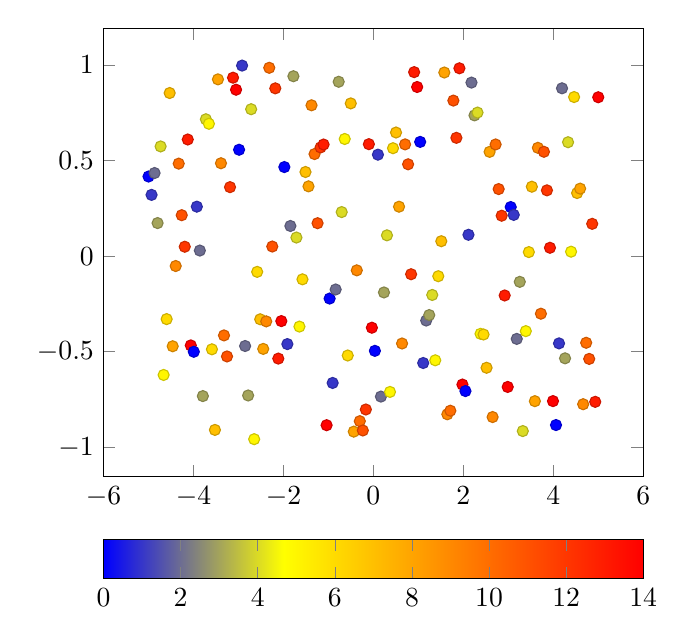
\begin{tikzpicture}
      \begin{axis}[colorbar horizontal]
        \addplot[only marks,scatter,
          scatter src={mod(\coordindex,15)},samples=150]
          {rand};
      \end{axis}
  \end{tikzpicture}}

\end{frame}

\begin{frame}[t]

  \frametitle{Search-Based Testing}
  \framesubtitle{Use a fitness function to guide the search to ``good'' values}

  \vspace*{.25in}
  \hspace{.25in}
  \resizebox{3.5in}{!}{
    \begin{tikzpicture}
      \begin{axis}[
          domain=0:1,
          xmax=1,
          ymax=1,
        ]
        \addplot3[surf] {x*y};
        \addplot3[solarizedRebase0,/pgfplots/quiver,
            quiver/u=y,
            quiver/v=x,
            quiver/w=0,
            quiver/scale arrows=0.1,
          -stealth,samples=10] {1};
      \end{axis}
  \end{tikzpicture}}

\end{frame}

\begin{frame}
  \frametitle{Performance of Search-based Software Testing}
   \tikzstyle{proc} = [draw, thick, fill=solarizedViolet, text centered, rounded corners,
    text=solarizedRebase02, draw=solarizedViolet]

\tikzstyle{prochighlight} = [draw, thick, fill=solarizedOrange, text centered, rounded corners,
    text=solarizedRebase02, draw=solarizedOrange]

\tikzstyle{procold} = [draw, thick, fill=solarizedViolet!75, text centered, rounded corners,
    text=solarizedRebase02, draw=solarizedViolet!75]

\tikzstyle{procchanged} = [draw, thick, fill=solarizedViolet!75, text centered, rounded corners,
    text=solarizedRebase02, draw=solarizedViolet!75]

\tikzstyle{prochighlightold} = [draw, thick, fill=solarizedOrange!75, text centered, rounded corners,
    text=solarizedRebase02, draw=solarizedOrange!75]

\tikzstyle{prochighlightchanged} = [draw, thick, fill=solarizedYellow!75, text centered, rounded corners,
    text=solarizedRebase02, draw=solarizedYellow!75]

\tikzstyle{proctest} = [draw, thick, fill=solarizedOrange, text centered, rounded corners,
text=solarizedBase02, draw=solarizedOrange]

\tikzstyle{procnew} = [draw, thick, fill=solarizedGreen, text centered, rounded corners,
    text=solarizedRebase02, draw=solarizedGreen]

\tikzstyle{procyellow} = [draw, thick, fill=solarizedYellow, text centered, rounded corners,
    text=solarizedRebase02, draw=solarizedYellow]

\tikzstyle{procred} = [draw, thick, fill=solarizedRed, text centered, rounded corners,
    text=solarizedRebase02, draw=solarizedRed]

\tikzstyle{io} = [ellipse, draw, thick, fill=solarizedBlue, draw=solarizedBlue, text=solarizedRebase02]

\tikzstyle{iopass} = [ellipse, draw, thick, fill=solarizedGreen, draw=solarizedGreen, text=solarizedRebase02]
\tikzstyle{iofail} = [ellipse, draw, thick, fill=solarizedRed, draw=solarizedRed, text=solarizedRebase02]
\tikzstyle{iohighlight} = [ellipse, draw, thick, fill=solarizedYellow, draw=solarizedYellow,
    text=solarizedRebase02]

\tikzstyle{iofailother} = [ellipse, draw, thick, fill=solarizedYellow, draw=solarizedYellow,
    text=solarizedRebase02]
\tikzstyle{wrongoutput} = [ellipse, draw, thick, fill=solarizedCyan, draw=solarizedCyan, text=solarizedRebase02]

\tikzstyle{special} = [draw, thick, fill=solarizedGreen, text centered, draw=solarizedGreen,
    text=solarizedBase02]
\tikzstyle{specialOrange} = [draw, thick, fill=solarizedOrange, text centered, draw=solarizedOrange,
    text=solarizedBase02]
\tikzstyle{specialGreen} = [draw, thick, fill=solarizedGreen, text centered, draw=solarizedGreen,
    text=solarizedBase02]
\tikzstyle{specialYellow} = [draw, thick, fill=solarizedYellow, text centered, draw=solarizedYellow,
    text=solarizedBase02]

\tikzstyle{pass} = [draw, thick, fill=solarizedGreen, text centered, draw=solarizedGreen, text=solarizedRebase02]
\tikzstyle{fail} = [draw, thick, fill=solarizedRed, text centered, draw=solarizedRed, text=solarizedRebase02]

\tikzstyle{feature} = [draw, thick, fill=solarizedOrange, text centered, text=solarizedRebase02, draw=solarizedOrange]

   %!TEX root=kinneer_seke.tex
% mainfile: kinneer_seke.tex

%%%%%%%%%%%%%%%%%%%%%%%%%%%%%%%%%%%%%%%%%%%%%%%%%%%%%%%%%%%%%%%
% Arithmetic of the clock
% Author: Juan Luis Varona
% http://www.unirioja.es/cu/jvarona/
%%%<
%%%>
% :Title: Arithmetic of the clock
% :Author: Juan Luis Varona
%
% This example shows the products i times j for
% i and j from 0 to 11 by using arithmetic modulo 12,
% i.e., the so called arithmetic of the clock.
%

% The results of the products are represented both by
% the color of the clock and by the hand.
% Colors:

% \definecolor{clock0}{cmyk}{1,0,0,0} % cyan
\definecolor{clock0}{HTML}{CB4B16}

\definecolor{clock1}{cmyk}{0.75,0.25,0,0}
\definecolor{clock2}{cmyk}{0.5,0.5,0,0}

% \definecolor{clock3}{cmyk}{0.25,0.75,0,0}
\definecolor{clock3}{HTML}{DC322F}

\definecolor{clock4}{cmyk}{0,1,0,0} % magenta
\definecolor{clock5}{cmyk}{0,0.75,0.25,0}
\definecolor{clock6}{cmyk}{0,0,5,0.5,0}
\definecolor{clock7}{cmyk}{0,0.25,0.75,0}
\definecolor{clock8}{cmyk}{0,0,1,0} % yellow

% \definecolor{clock9}{cmyk}{0.25,0,0.75,0}
\definecolor{clock9}{HTML}{6C71C4}

\definecolor{clock10}{cmyk}{0.5,0,0.5,0}

% \definecolor{clock11}{cmyk}{0.75,0,0.25,0}
\definecolor{clock11}{HTML}{268BD2}

% x pos, y pos, color, hand position
\newcommand{\clock}[4]{%
  \begin{scope}[xshift=2.25*#1cm,yshift=2.25*#2cm]
  % \filldraw [fill=#3, line width=1.6pt] (0,0) circle (1cm); % simple fill (unused)
  % \draw[fill] (0,0) circle (1mm); % border (unused)
  \shadedraw [inner color=#3!30!white, outer color=#3!90!black,
    line width=1.6pt] (0,0) circle (1cm); % disk with shadow and border
  \foreach \angle in {0, 30, ..., 330}
    \draw[line width=1pt] (\angle:0.82cm) -- (\angle:1cm);
  \foreach \angle in {0,90,180,270}
    \draw[line width=1.3pt] (\angle:0.75cm) -- (\angle:1cm);
  \draw[line width=1.6pt] (0,0) -- (90-30*#4:0.6cm); % the hand
  \end{scope}
}

\setbeamercovered{invisible}

\hspace*{.125in}
\begin{overprint}[5.0in]
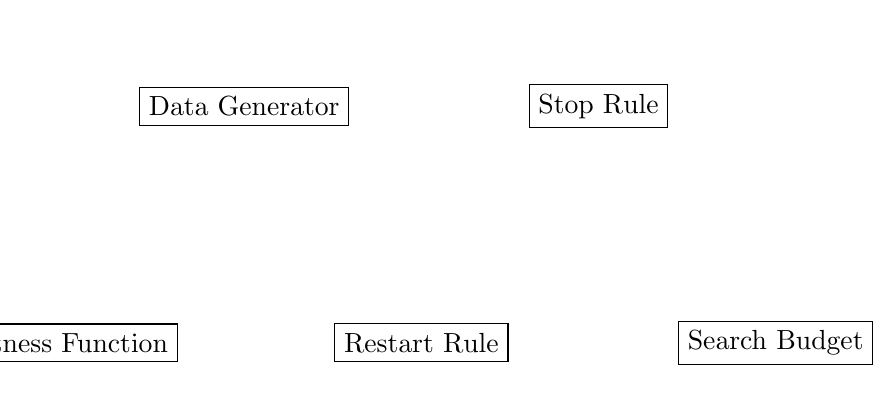
\begin{tikzpicture}[scale=1]

  \path[use as bounding box] (-0.5,2.5) rectangle (10,-2);

  \uncover<2->{
    \clock{0}{0}{clock0}{8};
    \node[draw] at (0cm,-1.5cm) {Fitness Function};
  }
  \uncover<3->{
    \clock{1}{0}{clock3}{1};
    \node[draw] at (2.25cm,+1.5cm) {Data Generator};
  }
  \uncover<4->{
    \clock{2}{0}{clock6}{6};
    \node[draw] at (4.50cm,-1.5cm) {Restart Rule};
  }
  \uncover<5->{
    \clock{3}{0}{clock9}{11};
    \node[draw] at (6.75cm,+1.5cm) {Stop Rule};
  }
  \uncover<6->{
    \clock{4}{0}{clock11}{10};
    \node[draw] at (9cm,-1.5cm) {Search Budget};
  }

\end{tikzpicture}

\hspace*{.33in}
\begin{tikzpicture}
  \path[use as bounding box] (-4.5,1) rectangle (10,-2);
  \path[->]<7-> node[special, text width=26ex]
    (Requirements) at (0,-.6)
    {{\Large How do parameter values influence the efficiency of SBST?}};

\end{tikzpicture}

\end{overprint}

\end{frame}

\setbeamercovered{invisible}
\begin{frame}
    \frametitle{Search-based Software Testing}
    \begin{center}
  \fontsize{60}{72}\selectfont
  O(\uncover<2->{?})
  \end{center}
  \tikzstyle{proc} = [draw, thick, fill=solarizedViolet, text centered, rounded corners,
    text=solarizedRebase02, draw=solarizedViolet]

\tikzstyle{prochighlight} = [draw, thick, fill=solarizedOrange, text centered, rounded corners,
    text=solarizedRebase02, draw=solarizedOrange]

\tikzstyle{procold} = [draw, thick, fill=solarizedViolet!75, text centered, rounded corners,
    text=solarizedRebase02, draw=solarizedViolet!75]

\tikzstyle{procchanged} = [draw, thick, fill=solarizedViolet!75, text centered, rounded corners,
    text=solarizedRebase02, draw=solarizedViolet!75]

\tikzstyle{prochighlightold} = [draw, thick, fill=solarizedOrange!75, text centered, rounded corners,
    text=solarizedRebase02, draw=solarizedOrange!75]

\tikzstyle{prochighlightchanged} = [draw, thick, fill=solarizedYellow!75, text centered, rounded corners,
    text=solarizedRebase02, draw=solarizedYellow!75]

\tikzstyle{proctest} = [draw, thick, fill=solarizedOrange, text centered, rounded corners,
text=solarizedBase02, draw=solarizedOrange]

\tikzstyle{procnew} = [draw, thick, fill=solarizedGreen, text centered, rounded corners,
    text=solarizedRebase02, draw=solarizedGreen]

\tikzstyle{procyellow} = [draw, thick, fill=solarizedYellow, text centered, rounded corners,
    text=solarizedRebase02, draw=solarizedYellow]

\tikzstyle{procred} = [draw, thick, fill=solarizedRed, text centered, rounded corners,
    text=solarizedRebase02, draw=solarizedRed]

\tikzstyle{io} = [ellipse, draw, thick, fill=solarizedBlue, draw=solarizedBlue, text=solarizedRebase02]

\tikzstyle{iopass} = [ellipse, draw, thick, fill=solarizedGreen, draw=solarizedGreen, text=solarizedRebase02]
\tikzstyle{iofail} = [ellipse, draw, thick, fill=solarizedRed, draw=solarizedRed, text=solarizedRebase02]
\tikzstyle{iohighlight} = [ellipse, draw, thick, fill=solarizedYellow, draw=solarizedYellow,
    text=solarizedRebase02]

\tikzstyle{iofailother} = [ellipse, draw, thick, fill=solarizedYellow, draw=solarizedYellow,
    text=solarizedRebase02]
\tikzstyle{wrongoutput} = [ellipse, draw, thick, fill=solarizedCyan, draw=solarizedCyan, text=solarizedRebase02]

\tikzstyle{special} = [draw, thick, fill=solarizedGreen, text centered, draw=solarizedGreen,
    text=solarizedBase02]
\tikzstyle{specialOrange} = [draw, thick, fill=solarizedOrange, text centered, draw=solarizedOrange,
    text=solarizedBase02]
\tikzstyle{specialGreen} = [draw, thick, fill=solarizedGreen, text centered, draw=solarizedGreen,
    text=solarizedBase02]
\tikzstyle{specialYellow} = [draw, thick, fill=solarizedYellow, text centered, draw=solarizedYellow,
    text=solarizedBase02]

\tikzstyle{pass} = [draw, thick, fill=solarizedGreen, text centered, draw=solarizedGreen, text=solarizedRebase02]
\tikzstyle{fail} = [draw, thick, fill=solarizedRed, text centered, draw=solarizedRed, text=solarizedRebase02]

\tikzstyle{feature} = [draw, thick, fill=solarizedOrange, text centered, text=solarizedRebase02, draw=solarizedOrange]

  \begin{tikzpicture}
          \path[->]<3-> node[special,]
                      (Requirements) at (1.5,.75)
              {Set of Program Methods $M = \{ M_1, M_2, \ldots, M_{11}, M_{12} \}$};
  \end{tikzpicture}
\end{frame}

  %background
  \section{Background}

    \begin{frame}
      \frametitle{Doubling Experiment}
    \end{frame}

    \section{Technique}
      \begin{frame}
        % \begin{figure}
          \frametitle{Method of Approach}
          \centering
          \tikzstyle{proc} = [draw, thick, fill=solarizedViolet, text centered, rounded corners,
    text=solarizedRebase02, draw=solarizedViolet]

\tikzstyle{prochighlight} = [draw, thick, fill=solarizedOrange, text centered, rounded corners,
    text=solarizedRebase02, draw=solarizedOrange]

\tikzstyle{procold} = [draw, thick, fill=solarizedViolet!75, text centered, rounded corners,
    text=solarizedRebase02, draw=solarizedViolet!75]

\tikzstyle{procchanged} = [draw, thick, fill=solarizedViolet!75, text centered, rounded corners,
    text=solarizedRebase02, draw=solarizedViolet!75]

\tikzstyle{prochighlightold} = [draw, thick, fill=solarizedOrange!75, text centered, rounded corners,
    text=solarizedRebase02, draw=solarizedOrange!75]

\tikzstyle{prochighlightchanged} = [draw, thick, fill=solarizedYellow!75, text centered, rounded corners,
    text=solarizedRebase02, draw=solarizedYellow!75]

\tikzstyle{proctest} = [draw, thick, fill=solarizedOrange, text centered, rounded corners,
text=solarizedBase02, draw=solarizedOrange]

\tikzstyle{procnew} = [draw, thick, fill=solarizedGreen, text centered, rounded corners,
    text=solarizedRebase02, draw=solarizedGreen]

\tikzstyle{procyellow} = [draw, thick, fill=solarizedYellow, text centered, rounded corners,
    text=solarizedRebase02, draw=solarizedYellow]

\tikzstyle{procred} = [draw, thick, fill=solarizedRed, text centered, rounded corners,
    text=solarizedRebase02, draw=solarizedRed]

\tikzstyle{io} = [ellipse, draw, thick, fill=solarizedBlue, draw=solarizedBlue, text=solarizedRebase02]

\tikzstyle{iopass} = [ellipse, draw, thick, fill=solarizedGreen, draw=solarizedGreen, text=solarizedRebase02]
\tikzstyle{iofail} = [ellipse, draw, thick, fill=solarizedRed, draw=solarizedRed, text=solarizedRebase02]
\tikzstyle{iohighlight} = [ellipse, draw, thick, fill=solarizedYellow, draw=solarizedYellow,
    text=solarizedRebase02]

\tikzstyle{iofailother} = [ellipse, draw, thick, fill=solarizedYellow, draw=solarizedYellow,
    text=solarizedRebase02]
\tikzstyle{wrongoutput} = [ellipse, draw, thick, fill=solarizedCyan, draw=solarizedCyan, text=solarizedRebase02]

\tikzstyle{special} = [draw, thick, fill=solarizedGreen, text centered, draw=solarizedGreen,
    text=solarizedBase02]
\tikzstyle{specialOrange} = [draw, thick, fill=solarizedOrange, text centered, draw=solarizedOrange,
    text=solarizedBase02]
\tikzstyle{specialGreen} = [draw, thick, fill=solarizedGreen, text centered, draw=solarizedGreen,
    text=solarizedBase02]
\tikzstyle{specialYellow} = [draw, thick, fill=solarizedYellow, text centered, draw=solarizedYellow,
    text=solarizedBase02]

\tikzstyle{pass} = [draw, thick, fill=solarizedGreen, text centered, draw=solarizedGreen, text=solarizedRebase02]
\tikzstyle{fail} = [draw, thick, fill=solarizedRed, text centered, draw=solarizedRed, text=solarizedRebase02]

\tikzstyle{feature} = [draw, thick, fill=solarizedOrange, text centered, text=solarizedRebase02, draw=solarizedOrange]

          \newcommand{\mx}[1]{\mathbf{\bm{#1}}} % Matrix command
\newcommand{\vc}[1]{\mathbf{\bm{#1}}} % Vector command

% Define the layers to draw the diagram
\pgfdeclarelayer{background}
\pgfdeclarelayer{foreground}
\pgfsetlayers{background,main,foreground}

% Define distances for bordering
\def\blockdist{3.5}
\def\vertdist{2}

\hspace{-.25in}

\begin{minipage}{5in}

  \begin{center}

    \vspace*{-.3in}
    \begin{minipage}{4.5in}

      \begin{figure}

        \begin{center}

\begin{tikzpicture}[thick,scale=1, every node/.style={scale=1}]

  \path[use as bounding box] (-3.0,2.5) rectangle (10,-2);

    \path[->]<1-> node[proc, text width=15ex]
    (sa) at (1.5,.75) {\centering \textit{SchemaAnalyst} \\ Execution};

    \path[->]<2-> node[io, left of=sa, yshift=0.70in, xshift=-1.25in,text width=7ex]
    (cc) {\centering Coverage \\ Criterion} (cc) edge node {} (sa);

    \path[->]<3-> node[io, left of=sa, yshift=0.0in, xshift=-1.25in,text width=7ex]
    (dg) {\centering Data \\ Generator} (dg) edge node {} (sa);

    \path[->]<4-6> node[io, left of=sa, yshift=-0.70in, xshift=-1.25in,text width=7ex]
    (ds) {\centering Database \\ Schema} (ds) edge node {} (sa);

    \path[->]<5> node[io, right of=sa, yshift=0.0in, xshift=1.25in,text width=7ex]
    (ts) {\centering Test \\ Suite \\} (sa) edge node {} (ts);

    \path[->]<6-> node[io, right of=sa, yshift=0.0in, xshift=1.25in,text width=7ex]
    (ts) {\centering Runtime} (sa) edge node {} (ts);

    \path[->]<7-> node[proc, below of=sa, yshift=-0.3in, xshift=0.0in,text width=15ex]
    (sd) {\centering Schema Doubler} (sd) edge node {Provides Schema} (sa);

    \path[->]<7-> node[io, left of=sa, yshift=-0.70in, xshift=-1.25in,text width=7ex]
    (ds) {\centering Database \\ Schema} (ds) edge node {} (sd);

    \path[->]<8-> node[io, left of=sa, yshift=-1.40in, xshift=-1.25in,text width=7ex]
    (dc) {\centering Doubler \\ Choice} (dc) edge node {} (sd);

    \path[->]<9-> node[proc, right of=sd, yshift=0.0in, xshift=1.25in,text width=15ex]
    (ca) {\centering Convergence \\ Algorithm} (ca) edge node [below=.20in]{Continue?} (sd);

    \path[->]<9-> (ts) edge node {} (ca);


\end{tikzpicture}

\end{center}

\end{figure}

\end{minipage}

\end{center}

\end{minipage}

        % \end{figure}
      \end{frame}

      \begin{frame}
        \frametitle{Doubling Database Schemas}
        \centering
        \tikzstyle{proc} = [draw, thick, fill=solarizedViolet, text centered, rounded corners,
    text=solarizedRebase02, draw=solarizedViolet]

\tikzstyle{prochighlight} = [draw, thick, fill=solarizedOrange, text centered, rounded corners,
    text=solarizedRebase02, draw=solarizedOrange]

\tikzstyle{procold} = [draw, thick, fill=solarizedViolet!75, text centered, rounded corners,
    text=solarizedRebase02, draw=solarizedViolet!75]

\tikzstyle{procchanged} = [draw, thick, fill=solarizedViolet!75, text centered, rounded corners,
    text=solarizedRebase02, draw=solarizedViolet!75]

\tikzstyle{prochighlightold} = [draw, thick, fill=solarizedOrange!75, text centered, rounded corners,
    text=solarizedRebase02, draw=solarizedOrange!75]

\tikzstyle{prochighlightchanged} = [draw, thick, fill=solarizedYellow!75, text centered, rounded corners,
    text=solarizedRebase02, draw=solarizedYellow!75]

\tikzstyle{proctest} = [draw, thick, fill=solarizedOrange, text centered, rounded corners,
text=solarizedBase02, draw=solarizedOrange]

\tikzstyle{procnew} = [draw, thick, fill=solarizedGreen, text centered, rounded corners,
    text=solarizedRebase02, draw=solarizedGreen]

\tikzstyle{procyellow} = [draw, thick, fill=solarizedYellow, text centered, rounded corners,
    text=solarizedRebase02, draw=solarizedYellow]

\tikzstyle{procred} = [draw, thick, fill=solarizedRed, text centered, rounded corners,
    text=solarizedRebase02, draw=solarizedRed]

\tikzstyle{io} = [ellipse, draw, thick, fill=solarizedBlue, draw=solarizedBlue, text=solarizedRebase02]

\tikzstyle{iopass} = [ellipse, draw, thick, fill=solarizedGreen, draw=solarizedGreen, text=solarizedRebase02]
\tikzstyle{iofail} = [ellipse, draw, thick, fill=solarizedRed, draw=solarizedRed, text=solarizedRebase02]
\tikzstyle{iohighlight} = [ellipse, draw, thick, fill=solarizedYellow, draw=solarizedYellow,
    text=solarizedRebase02]

\tikzstyle{iofailother} = [ellipse, draw, thick, fill=solarizedYellow, draw=solarizedYellow,
    text=solarizedRebase02]
\tikzstyle{wrongoutput} = [ellipse, draw, thick, fill=solarizedCyan, draw=solarizedCyan, text=solarizedRebase02]

\tikzstyle{special} = [draw, thick, fill=solarizedGreen, text centered, draw=solarizedGreen,
    text=solarizedBase02]
\tikzstyle{specialOrange} = [draw, thick, fill=solarizedOrange, text centered, draw=solarizedOrange,
    text=solarizedBase02]
\tikzstyle{specialGreen} = [draw, thick, fill=solarizedGreen, text centered, draw=solarizedGreen,
    text=solarizedBase02]
\tikzstyle{specialYellow} = [draw, thick, fill=solarizedYellow, text centered, draw=solarizedYellow,
    text=solarizedBase02]

\tikzstyle{pass} = [draw, thick, fill=solarizedGreen, text centered, draw=solarizedGreen, text=solarizedRebase02]
\tikzstyle{fail} = [draw, thick, fill=solarizedRed, text centered, draw=solarizedRed, text=solarizedRebase02]

\tikzstyle{feature} = [draw, thick, fill=solarizedOrange, text centered, text=solarizedRebase02, draw=solarizedOrange]

        %!TEX root=kinneer_seke.tex
% mainfile: kinneer_seke.tex

\pgfdeclarelayer{background}
\pgfdeclarelayer{foreground}
\pgfsetlayers{background,main,foreground}

\begin{minipage}{.5in}

\begin{center}

\begin{minipage}{.45in}

  \vspace*{-.4in}
\begin{figure}

\begin{center}

  \hspace*{-2.25in}
\begin{tikzpicture}[thick,scale=1.3, every node/.style={scale=1}]

\path[use as bounding box] (-5.0,2.5) rectangle (10,-2);

\node<1-> (table) [proc] {
    \begin{tabular}{l}
    \textbf{Table}\\ \hline
        \parbox{4cm}{
            \begin{itemize}
                \color{solarizedBase02}
                \item Column 1
                \item Column 2
                \item \dots
                \item Column n
            \end{itemize}
        }
    \end{tabular}
};

\path<2-> (table.west)+(-2,0) node (nn1) [proctest] {NOT NULL};
\path<2-> [draw, ->] (nn1.east) -- node [above] {} (table.179);

\path[->]<3-> node[proctest, right of=table, yshift=0.0in,xshift=1.25in, minimum width=7ex] (pkey) {PRIMARY KEY} (pkey.west) edge node {} (table.340);

\path[->]<4-> node[proctest, above of=nn1, yshift=0.0in, xshift=0.0in, minimum width=7ex] (unique) {UNIQUE} (unique.east) edge node {} (table);

\path[->]<5-> node[proctest, below of=pkey, yshift=0.0in, xshift=0.0in, minimum width=7ex] (check) {CHECK} (check.west) edge node {} (table);

\path[->]<6-> node[proctest, above of=pkey, yshift=0.0in, xshift=0.0in, minimum width=7ex] (fkey) {FORIEGN KEY} (fkey.west) edge node {} (table);

\path[->]<6-> node[proc, above of=fkey, yshift=0.0in, xshift=1.5in,
minimum width=7ex] (rtab) {} (rtab) edge node {} (fkey.east);

\path<7-> (nn1.south)+(0,-.5) node (nn2) [proctest] {NOT NULL};
\path<7-> [draw, ->] (nn2.east) -- node [above] {} (table.181);

\end{tikzpicture}

\end{center}
\end{figure}
\end{minipage}
\end{center}
\end{minipage}

      \end{frame}

    \section{Experiment Design}

      \begin{frame}
        \frametitle{Experiments}
        \centering
        \tikzstyle{proc} = [draw, thick, fill=solarizedViolet, text centered, rounded corners,
    text=solarizedRebase02, draw=solarizedViolet]

\tikzstyle{prochighlight} = [draw, thick, fill=solarizedOrange, text centered, rounded corners,
    text=solarizedRebase02, draw=solarizedOrange]

\tikzstyle{procold} = [draw, thick, fill=solarizedViolet!75, text centered, rounded corners,
    text=solarizedRebase02, draw=solarizedViolet!75]

\tikzstyle{procchanged} = [draw, thick, fill=solarizedViolet!75, text centered, rounded corners,
    text=solarizedRebase02, draw=solarizedViolet!75]

\tikzstyle{prochighlightold} = [draw, thick, fill=solarizedOrange!75, text centered, rounded corners,
    text=solarizedRebase02, draw=solarizedOrange!75]

\tikzstyle{prochighlightchanged} = [draw, thick, fill=solarizedYellow!75, text centered, rounded corners,
    text=solarizedRebase02, draw=solarizedYellow!75]

\tikzstyle{proctest} = [draw, thick, fill=solarizedOrange, text centered, rounded corners,
text=solarizedBase02, draw=solarizedOrange]

\tikzstyle{procnew} = [draw, thick, fill=solarizedGreen, text centered, rounded corners,
    text=solarizedRebase02, draw=solarizedGreen]

\tikzstyle{procyellow} = [draw, thick, fill=solarizedYellow, text centered, rounded corners,
    text=solarizedRebase02, draw=solarizedYellow]

\tikzstyle{procred} = [draw, thick, fill=solarizedRed, text centered, rounded corners,
    text=solarizedRebase02, draw=solarizedRed]

\tikzstyle{io} = [ellipse, draw, thick, fill=solarizedBlue, draw=solarizedBlue, text=solarizedRebase02]

\tikzstyle{iopass} = [ellipse, draw, thick, fill=solarizedGreen, draw=solarizedGreen, text=solarizedRebase02]
\tikzstyle{iofail} = [ellipse, draw, thick, fill=solarizedRed, draw=solarizedRed, text=solarizedRebase02]
\tikzstyle{iohighlight} = [ellipse, draw, thick, fill=solarizedYellow, draw=solarizedYellow,
    text=solarizedRebase02]

\tikzstyle{iofailother} = [ellipse, draw, thick, fill=solarizedYellow, draw=solarizedYellow,
    text=solarizedRebase02]
\tikzstyle{wrongoutput} = [ellipse, draw, thick, fill=solarizedCyan, draw=solarizedCyan, text=solarizedRebase02]

\tikzstyle{special} = [draw, thick, fill=solarizedGreen, text centered, draw=solarizedGreen,
    text=solarizedBase02]
\tikzstyle{specialOrange} = [draw, thick, fill=solarizedOrange, text centered, draw=solarizedOrange,
    text=solarizedBase02]
\tikzstyle{specialGreen} = [draw, thick, fill=solarizedGreen, text centered, draw=solarizedGreen,
    text=solarizedBase02]
\tikzstyle{specialYellow} = [draw, thick, fill=solarizedYellow, text centered, draw=solarizedYellow,
    text=solarizedBase02]

\tikzstyle{pass} = [draw, thick, fill=solarizedGreen, text centered, draw=solarizedGreen, text=solarizedRebase02]
\tikzstyle{fail} = [draw, thick, fill=solarizedRed, text centered, draw=solarizedRed, text=solarizedRebase02]

\tikzstyle{feature} = [draw, thick, fill=solarizedOrange, text centered, text=solarizedRebase02, draw=solarizedOrange]

        \begin{tikzpicture}[node distance=0cm, auto,>=stealth, thick]

        \path[use as bounding box] (-2,4.5) rectangle (10,-2);

        % Computer Software
        \path[->]<1-> node[proc, text width=14ex]
        (Software) at (3.5,2.5) {Experimental Parameters};

        % Code
        \path[->]<2-> node[proc, right of=Software,
                      yshift=-.5in, xshift=-1.75in, text width=12ex]
                      (Code) {Coverage Criterion}
        (Software) edge node {} (Code);

        % Features
        \path[->]<3-> node[proc, below of=Software,
                      yshift=-1in, xshift=-.75in, text width=12ex]
                      (Features) {Data \\ Generator}
        (Software) edge node {} (Features);

        % Feature Interactions
        \path[->]<4-> node[proc, below of=Software,
                      yshift=-1in, xshift=.75in, text width=12ex]
                      (Interactions) {Doubling \\ Technique}
        (Software) edge node {} (Interactions);

        % Execution Environments
        \path[->]<5-> node[proc, right of=Software,
                      yshift=-.5in, xshift=1.75in, text width=12ex]
                      (Environment) {Database \\ Schema}
        (Software) edge node {} (Environment);

                % Brooks Quotation
        \path[->]<6-> node[specialGreen, below of=Software,
                      yshift=-1.5in,text width=40ex]
                      (Quotations)
                      {Over 2,000 combinations!};

        \path[->]<7-> node[specialGreen, below of=Quotations,
                      yshift=-0.4in,text width=40ex]
                      (conclusion)
                      {Experiments ran on HPC cluster with 3440 cores.};

\end{tikzpicture}

      \end{frame}

      \begin{frame}
        \frametitle{Experiments}
        \begin{columns}
        \column{0.5\textwidth}
        \begin{itemize}
          \item Parameters Studied
          \item Cluster
        \end{itemize}
          \column{0.5\textwidth}
          \begin{figure}
            \includegraphics[width=\textwidth]{iceberg2014.jpg}
          \end{figure}
      \end{columns}
      \end{frame}

         \begin{frame}
        \frametitle{Experiments}
        \centering
        \tikzstyle{proc} = [draw, thick, fill=solarizedViolet, text centered, rounded corners,
    text=solarizedRebase02, draw=solarizedViolet]

\tikzstyle{prochighlight} = [draw, thick, fill=solarizedOrange, text centered, rounded corners,
    text=solarizedRebase02, draw=solarizedOrange]

\tikzstyle{procold} = [draw, thick, fill=solarizedViolet!75, text centered, rounded corners,
    text=solarizedRebase02, draw=solarizedViolet!75]

\tikzstyle{procchanged} = [draw, thick, fill=solarizedViolet!75, text centered, rounded corners,
    text=solarizedRebase02, draw=solarizedViolet!75]

\tikzstyle{prochighlightold} = [draw, thick, fill=solarizedOrange!75, text centered, rounded corners,
    text=solarizedRebase02, draw=solarizedOrange!75]

\tikzstyle{prochighlightchanged} = [draw, thick, fill=solarizedYellow!75, text centered, rounded corners,
    text=solarizedRebase02, draw=solarizedYellow!75]

\tikzstyle{proctest} = [draw, thick, fill=solarizedOrange, text centered, rounded corners,
text=solarizedBase02, draw=solarizedOrange]

\tikzstyle{procnew} = [draw, thick, fill=solarizedGreen, text centered, rounded corners,
    text=solarizedRebase02, draw=solarizedGreen]

\tikzstyle{procyellow} = [draw, thick, fill=solarizedYellow, text centered, rounded corners,
    text=solarizedRebase02, draw=solarizedYellow]

\tikzstyle{procred} = [draw, thick, fill=solarizedRed, text centered, rounded corners,
    text=solarizedRebase02, draw=solarizedRed]

\tikzstyle{io} = [ellipse, draw, thick, fill=solarizedBlue, draw=solarizedBlue, text=solarizedRebase02]

\tikzstyle{iopass} = [ellipse, draw, thick, fill=solarizedGreen, draw=solarizedGreen, text=solarizedRebase02]
\tikzstyle{iofail} = [ellipse, draw, thick, fill=solarizedRed, draw=solarizedRed, text=solarizedRebase02]
\tikzstyle{iohighlight} = [ellipse, draw, thick, fill=solarizedYellow, draw=solarizedYellow,
    text=solarizedRebase02]

\tikzstyle{iofailother} = [ellipse, draw, thick, fill=solarizedYellow, draw=solarizedYellow,
    text=solarizedRebase02]
\tikzstyle{wrongoutput} = [ellipse, draw, thick, fill=solarizedCyan, draw=solarizedCyan, text=solarizedRebase02]

\tikzstyle{special} = [draw, thick, fill=solarizedGreen, text centered, draw=solarizedGreen,
    text=solarizedBase02]
\tikzstyle{specialOrange} = [draw, thick, fill=solarizedOrange, text centered, draw=solarizedOrange,
    text=solarizedBase02]
\tikzstyle{specialGreen} = [draw, thick, fill=solarizedGreen, text centered, draw=solarizedGreen,
    text=solarizedBase02]
\tikzstyle{specialYellow} = [draw, thick, fill=solarizedYellow, text centered, draw=solarizedYellow,
    text=solarizedBase02]

\tikzstyle{pass} = [draw, thick, fill=solarizedGreen, text centered, draw=solarizedGreen, text=solarizedRebase02]
\tikzstyle{fail} = [draw, thick, fill=solarizedRed, text centered, draw=solarizedRed, text=solarizedRebase02]

\tikzstyle{feature} = [draw, thick, fill=solarizedOrange, text centered, text=solarizedRebase02, draw=solarizedOrange]

        \begin{tikzpicture}[node distance=0cm, auto,>=stealth, thick]

        \path[use as bounding box] (-2,4.5) rectangle (10,-2);

        % Computer Software
        \path[->]<1-> node[io, minimum width=10ex]
        (Software) at (3.5,2.5) {Tables};

        % Features
        \path[->]<3-> node[io, below of=Software,
                      yshift=-1in, xshift=-.75in, minimum width=10ex]
                      (Features) {Criterion}
        (Software) edge node {} (Features);

        % Feature Interactions
        \path[->]<4-> node[io, below of=Software,
                      yshift=-1in, xshift=.75in, minimum width=10ex]
                      (Interactions) {Tables}
        (Software) edge node {} (Interactions);

                      % Brooks Quotation
        \path[->]<5-> node[specialGreen, below of=Software,
                      yshift=-1.5in,text width=40ex]
                      (Quotations)
                      {Too many combinations!};

\end{tikzpicture}

      \end{frame}

      \begin{frame}
        \frametitle{Criterion}
        \includegraphics[width=\textwidth]{CriterionBox}
        \tikzstyle{proc} = [draw, thick, fill=solarizedViolet, text centered, rounded corners,
    text=solarizedRebase02, draw=solarizedViolet]

\tikzstyle{prochighlight} = [draw, thick, fill=solarizedOrange, text centered, rounded corners,
    text=solarizedRebase02, draw=solarizedOrange]

\tikzstyle{procold} = [draw, thick, fill=solarizedViolet!75, text centered, rounded corners,
    text=solarizedRebase02, draw=solarizedViolet!75]

\tikzstyle{procchanged} = [draw, thick, fill=solarizedViolet!75, text centered, rounded corners,
    text=solarizedRebase02, draw=solarizedViolet!75]

\tikzstyle{prochighlightold} = [draw, thick, fill=solarizedOrange!75, text centered, rounded corners,
    text=solarizedRebase02, draw=solarizedOrange!75]

\tikzstyle{prochighlightchanged} = [draw, thick, fill=solarizedYellow!75, text centered, rounded corners,
    text=solarizedRebase02, draw=solarizedYellow!75]

\tikzstyle{proctest} = [draw, thick, fill=solarizedOrange, text centered, rounded corners,
text=solarizedBase02, draw=solarizedOrange]

\tikzstyle{procnew} = [draw, thick, fill=solarizedGreen, text centered, rounded corners,
    text=solarizedRebase02, draw=solarizedGreen]

\tikzstyle{procyellow} = [draw, thick, fill=solarizedYellow, text centered, rounded corners,
    text=solarizedRebase02, draw=solarizedYellow]

\tikzstyle{procred} = [draw, thick, fill=solarizedRed, text centered, rounded corners,
    text=solarizedRebase02, draw=solarizedRed]

\tikzstyle{io} = [ellipse, draw, thick, fill=solarizedBlue, draw=solarizedBlue, text=solarizedRebase02]

\tikzstyle{iopass} = [ellipse, draw, thick, fill=solarizedGreen, draw=solarizedGreen, text=solarizedRebase02]
\tikzstyle{iofail} = [ellipse, draw, thick, fill=solarizedRed, draw=solarizedRed, text=solarizedRebase02]
\tikzstyle{iohighlight} = [ellipse, draw, thick, fill=solarizedYellow, draw=solarizedYellow,
    text=solarizedRebase02]

\tikzstyle{iofailother} = [ellipse, draw, thick, fill=solarizedYellow, draw=solarizedYellow,
    text=solarizedRebase02]
\tikzstyle{wrongoutput} = [ellipse, draw, thick, fill=solarizedCyan, draw=solarizedCyan, text=solarizedRebase02]

\tikzstyle{special} = [draw, thick, fill=solarizedGreen, text centered, draw=solarizedGreen,
    text=solarizedBase02]
\tikzstyle{specialOrange} = [draw, thick, fill=solarizedOrange, text centered, draw=solarizedOrange,
    text=solarizedBase02]
\tikzstyle{specialGreen} = [draw, thick, fill=solarizedGreen, text centered, draw=solarizedGreen,
    text=solarizedBase02]
\tikzstyle{specialYellow} = [draw, thick, fill=solarizedYellow, text centered, draw=solarizedYellow,
    text=solarizedBase02]

\tikzstyle{pass} = [draw, thick, fill=solarizedGreen, text centered, draw=solarizedGreen, text=solarizedRebase02]
\tikzstyle{fail} = [draw, thick, fill=solarizedRed, text centered, draw=solarizedRed, text=solarizedRebase02]

\tikzstyle{feature} = [draw, thick, fill=solarizedOrange, text centered, text=solarizedRebase02, draw=solarizedOrange]

        \begin{tikzpicture}
          \path[->]<3-> node[special,]
                      (Requirements) at (1.5,.75)
              {Set of Program Methods $M = \{ M_1, M_2, \ldots, M_{11}, M_{12} \}$};
  \end{tikzpicture}

      \end{frame}

      \begin{frame}
        \frametitle{Data Generator}
        \includegraphics[width=\textwidth]{DataGeneratorBox}
        \tikzstyle{proc} = [draw, thick, fill=solarizedViolet, text centered, rounded corners,
    text=solarizedRebase02, draw=solarizedViolet]

\tikzstyle{prochighlight} = [draw, thick, fill=solarizedOrange, text centered, rounded corners,
    text=solarizedRebase02, draw=solarizedOrange]

\tikzstyle{procold} = [draw, thick, fill=solarizedViolet!75, text centered, rounded corners,
    text=solarizedRebase02, draw=solarizedViolet!75]

\tikzstyle{procchanged} = [draw, thick, fill=solarizedViolet!75, text centered, rounded corners,
    text=solarizedRebase02, draw=solarizedViolet!75]

\tikzstyle{prochighlightold} = [draw, thick, fill=solarizedOrange!75, text centered, rounded corners,
    text=solarizedRebase02, draw=solarizedOrange!75]

\tikzstyle{prochighlightchanged} = [draw, thick, fill=solarizedYellow!75, text centered, rounded corners,
    text=solarizedRebase02, draw=solarizedYellow!75]

\tikzstyle{proctest} = [draw, thick, fill=solarizedOrange, text centered, rounded corners,
text=solarizedBase02, draw=solarizedOrange]

\tikzstyle{procnew} = [draw, thick, fill=solarizedGreen, text centered, rounded corners,
    text=solarizedRebase02, draw=solarizedGreen]

\tikzstyle{procyellow} = [draw, thick, fill=solarizedYellow, text centered, rounded corners,
    text=solarizedRebase02, draw=solarizedYellow]

\tikzstyle{procred} = [draw, thick, fill=solarizedRed, text centered, rounded corners,
    text=solarizedRebase02, draw=solarizedRed]

\tikzstyle{io} = [ellipse, draw, thick, fill=solarizedBlue, draw=solarizedBlue, text=solarizedRebase02]

\tikzstyle{iopass} = [ellipse, draw, thick, fill=solarizedGreen, draw=solarizedGreen, text=solarizedRebase02]
\tikzstyle{iofail} = [ellipse, draw, thick, fill=solarizedRed, draw=solarizedRed, text=solarizedRebase02]
\tikzstyle{iohighlight} = [ellipse, draw, thick, fill=solarizedYellow, draw=solarizedYellow,
    text=solarizedRebase02]

\tikzstyle{iofailother} = [ellipse, draw, thick, fill=solarizedYellow, draw=solarizedYellow,
    text=solarizedRebase02]
\tikzstyle{wrongoutput} = [ellipse, draw, thick, fill=solarizedCyan, draw=solarizedCyan, text=solarizedRebase02]

\tikzstyle{special} = [draw, thick, fill=solarizedGreen, text centered, draw=solarizedGreen,
    text=solarizedBase02]
\tikzstyle{specialOrange} = [draw, thick, fill=solarizedOrange, text centered, draw=solarizedOrange,
    text=solarizedBase02]
\tikzstyle{specialGreen} = [draw, thick, fill=solarizedGreen, text centered, draw=solarizedGreen,
    text=solarizedBase02]
\tikzstyle{specialYellow} = [draw, thick, fill=solarizedYellow, text centered, draw=solarizedYellow,
    text=solarizedBase02]

\tikzstyle{pass} = [draw, thick, fill=solarizedGreen, text centered, draw=solarizedGreen, text=solarizedRebase02]
\tikzstyle{fail} = [draw, thick, fill=solarizedRed, text centered, draw=solarizedRed, text=solarizedRebase02]

\tikzstyle{feature} = [draw, thick, fill=solarizedOrange, text centered, text=solarizedRebase02, draw=solarizedOrange]

        \begin{tikzpicture}
          \path[->]<3-> node[special,]
                      (Requirements) at (1.5,.75)
              {Set of Program Methods $M = \{ M_1, M_2, \ldots, M_{11}, M_{12} \}$};
  \end{tikzpicture}

      \end{frame}


    \section{Conclusion}
      \begin{frame}
        \frametitle{Conclusion}
      \end{frame}

      % \begin{frame}
      %   \titlepage
      % \end{frame}

      \end{document}
